\subsection{Overview}

% \todo{
% the challenge of point cloud representation; from a high-level, how we are able to overcome the challenge
% 
% aside, the ambiguity of groundtruth is an inherent property of this problem; how do we resolve this problem.
% 
% describe the overall network architecture; give the road map for the rest of the section.
% }

Our task of building a conditional generative network for point sets is challenging, due to the unordered form of representation and the inherent ambiguity of groundtruth. These challenges has pushed us to invent new architecture, loss function, and learning paradigm. Specifically, we have to address three subproblems: 

\para{Point set generator architecture}: Network to predict point set is barely studied in literature, leaving a huge open space for us to explore the design choices. Ideally, a network should make the best use of its data statistics and possess enough representation power. We propose a network with two prediction branches, one enjoys high flexibility in capturing complicated structures and the other exploits geometric continuity. Its representation power is further boosted by an hourglass structure. See Sec~\ref{sec:method:network}. 

\para{Loss function for point set comparison}: For our novel type of prediction, point set, it is unclear how to measure the distance between the prediction and groundtruth. We introduce two distance metrics for point sets -- the Chamfer distance and the Earth Mover's distance. We show that both metrics are differentiable almost everywhere and can be used as the loss function, but has different properties in capturing shape space. See Sec~\ref{sec:method:loss}.

\para{Modeling the uncertainty of groundtruth}: Our problem of 3D structural recovery from a single image is ill-posed, thus the ambiguity of groundtruth arises during the train and test time. It is fundamentally important to characterize the ambiguity of groundtruth for a given input, and practically desirable to be able to generate multiple predictions. Surprisingly, this goal can be achieved tactfully by simply using the $\min$ function as a wrapper to the above proposed loss, or by a conditional variational autoencoder.  See Sec~\ref{sec:method:gan}.
% The form of the wrapper function is a $\min$ function of $n$ numbers. 
% The learning of this wrapped loss function (named {\bf MoN} loss) is almost as efficient and easy as the original one. 

% Here we choose the point cloud representation for 3D shapes --  a shape is a set of 3D coordinates $\mathcal{S}=\{(x_1, y_1, z_1),\dots, (x_n, y_n, z_n)\}$. By set, we mean a collection of \emph{orderless} entities.

% Most deep learning work predict either sequential data or 2D/3D arrays, thus there lacks literature on how point set should be represented and predicted. 

% Different from previous 3D deep learning work such as  that represent shapes by volume,
% Our system takes a single RGB or depth image as input, and is able to predict a list of a complete 3D point set as the candidate underlying 3D shape.

\subsection{Point Set Prediction Network}
\label{sec:method:network}
% \todo{
% describe the basic architecture of the point set predictor network;
% 
% describe the hour-glass network structure
% 
% describe the use of deconv branch and fc branch;
% }
The task of building a network for point set prediction is new. We design a network with the goal of possessing strong representation power for complicated structures, and make the best use of the statistics of geometric data. 
 % Next we introduce the basic ideas behind of our proposed network architecture. 
To introduce our network progressively, we start from a simple version and gradually add components.

% Given an image and a random vector as input, our point set prediction network ({\bf PointOutNet}) outputs a set of $N$ points in $\R^3$. This set is represented as an $N\times 3$ matrix, whose each row corresponds to a point.

As in Fig~\ref{fig:pointnet} (top), our network has an encoder stage and a predictor stage. The encoder maps the input pair of an image $\image$ and a random vector $r$ into an embedding space. The predictor outputs a shape as an $N\times 3$ matrix ${\bf M}$, each row containing the coordinates of one point.

The encoder is a composition of convolution and ReLU layers; in addition, a random vector $r$ is subsumed so that it perturbs the prediction from the image $I$. We postpone the explanation of how $r$ is used to Sec~\ref{sec:method:gan}. %This is done by first converting $r$ into a 3-dimensional tensor through fully-connected layers and a reshape layer, and then concatenating this tensor with the feature map of $I$, as in our supplementary. 
The predictor generates the coordinates of $N$ points through a fully connected network. Though simple, this version works reasonably well in practice. 

We further improve the design of the predictor branch to better accommodate large and smooth surfaces which are common in natural objects. The fully connected predictor as above cannot make full use of such natural geometric statistics, since each point is predicted independently. The improved predictor in Fig~\ref{fig:pointnet} (middle) exploits this geometric smoothness property. 

This version has two parallel predictor branches -- a fully-connected (fc) branch and a deconvolution (deconv) branch. The fc branch predicts $N_1$ points as before. The deconv branch predicts a 3 channel image of size $H\times W$, of which the three values at each pixel are the coordinates of a point, giving another $H\times W$ points. Their predictions are later merged together to form the whole set of points in ${\bf M}$. Multiple skip links are added to boost information flow across encoder and predictor. 

With the fc branch, our model enjoys high flexibility, showing good performance at describing intricate structures. With the deconvolution branch, our model becomes not only more parameter parsimonious by weight sharing; but also more friendly to large smooth surfaces, due to the spatial continuity induced by deconv and conv. Refer to Sec~\ref{sec:exp:analysis} for experimental evidences. 

To pursue even better performance, we introduce the hourglass version in Fig~\ref{fig:pointnet} (bottom), inspired by \cite{newell2016stacked}. This deep network conducts the encoding-decoding operations recurrently, thus has stronger representation power and can mix global and local information better. 

Above introduces the design of our network $\mathbb{G}$ in Eq~\ref{eqn:main}. To train this network, however, we still need to design a proper loss function for point set prediction, and enable the role $r$ for multiple candidates prediction. We explain in the next two sections.
\subsection{Distance Metric between Point Sets}
\label{sec:method:loss}



A critical challenge is to design a good loss function for comparing the predicted point cloud and the groundtruth. To plug in a neural network, a suitable distance must satisfy at least three conditions: 1) differentiable with respect to point locations; 2) efficient to compute, as data will be forwarded and back-propagated for many times; 3) robust against small number of outlier points in the sets (e.g. Hausdorff distance would fail).

We seek for a distance $d$ between subsets in $\R^3$, so that the loss function $L(\{S^{pred}_i\}, \{S^{gt}_i\})$ takes the form
\begin{align}
    L(\{S^{pred}_i\}, \{S^{gt}_i\}) = \sum d(S^{pred}_i, S^{gt}_i),
    \label{eqn:loss}
\end{align}
where $i$ indexes training samples, $S_i^{pred}$ and $S_i^{gt}$ are the prediction and groundtruth of each sample, respectively.

We propose two candidates: Chamfer distance (CD) and Earth Mover's distance (EMD)~\cite{rubner2000earth}.

\paragraph{Chamfer distance} We define the Chamfer distance between $S_1, S_2\subseteq \R^3$ as:
\begin{align*}
%\mathbb{D}_{\mbox{CD}}(S_1, S_2)=\frac{1}{|S_1|}\sum_{x\in S_1} \min_{y\in S_2} \|x-y\|_2+\frac{1}{|S_2|}\sum_{y\in S_2} \min_{x\in S_1} \|x-y\|_2
d_{CD}(S_1, S_2)=\sum_{x\in S_1}\min_{y\in S_2} \|x-y\|^2_2+\sum_{y\in S_2}\min_{x\in S_1} \|x-y\|^2_2
\end{align*}
In the strict sense, $d_{CD}$ is not a distance function because triangle inequality does not hold. We nevertheless use the term ``distance'' to refer to any non-negative function defined on point set pairs. For each point, the algorithm of CD finds the nearest neighbor in the other set and sums the squared distances up.   Viewed as a function of point locations in $S_1$ and $S_2$, $\mbox{CD}$ is continuous and piecewise smooth. The range search for each point is independent, thus trivially parallelizable. Also, spatial data structures like KD-tree can be used to accelerate nearest neighbor search. Though simple, CD produces reasonable high quality results in practice.

\paragraph{Earth Mover's distance} 

Consider $S_1, S_2\subseteq \R^3$ of equal size $s=|S_1|=|S_2|$. The EMD between $A$ and $B$ is defined as:
\begin{align*}
d_{EMD}(S_1, S_2)=\min_{\phi:S_1\rightarrow S_2} \sum_{x\in S_1} \|x-\phi(x)\|_2
\end{align*}
where $\phi:S_1\rightarrow S_2$ is a bijection.

The EMD distance solves an optimization problem, namely, the assignment problem. For all but a zero-measure subset of point set pairs, the optimal bijection $\phi$ is unique and invariant under infinitesimal movement of the points. Thus EMD is differentiable almost everywhere. In practice, exact computation of EMD is too expensive for deep learning, even on graphics hardware. We therefore implement a $(1+\epsilon)$ approximation scheme given by \cite{bertsekas1985distributed}. We allocate fix amount of time for each instance and incrementally adjust allowable error ratio to ensure termination. For typical inputs, the algorithm gives highly accurate results (approximation error on the magnitude of $1\%$). The algorithm is easily parallelizable on GPU.

%\paragraph{Shape space} Though more expensive to compute, the shape space induced by EMD is nicer than by CD. Fig~\ref{fig:interoplation} illustrates their differences in a shape interpolation simulation. Evidently, the mean shape by EMD is cleaner and clearer in structure. Intuitively, this is because the EMD is obtained through solving a point-wise correspondence problem, and the correspondence implicitly suggests the proper movement of each point for interpolation. In contrast, the mean shape from CD is more splashy, as CD takes a greedy algorithm (nearest neighbor) to match points, resulting in a strategy that tends to hedge the uncertainty in groundtruth by a few isolated points. 

%We are particularly interested in how point clouds will be averaged, because this precursors what our complicated network may learn. As will be discussed in more detail in the next section, 3D reconstruction from a single 2D image is inherently ambiguous. Such ambiguity affects the optimization of loss function (Eq~\ref{eqn:loss}), an objective that drives to average possible groundtruth shapes for each input. 

%In 3D reconstruction experiments, we do observe similar trends: Chamfer distance tends to induce a more ``aggressive'' reconstruction by placing a few points at uncertain space; in contrast, EMD tends to be more conservative and produce less spurious points.

%\begin{figure}[t!]
  %\centering
  %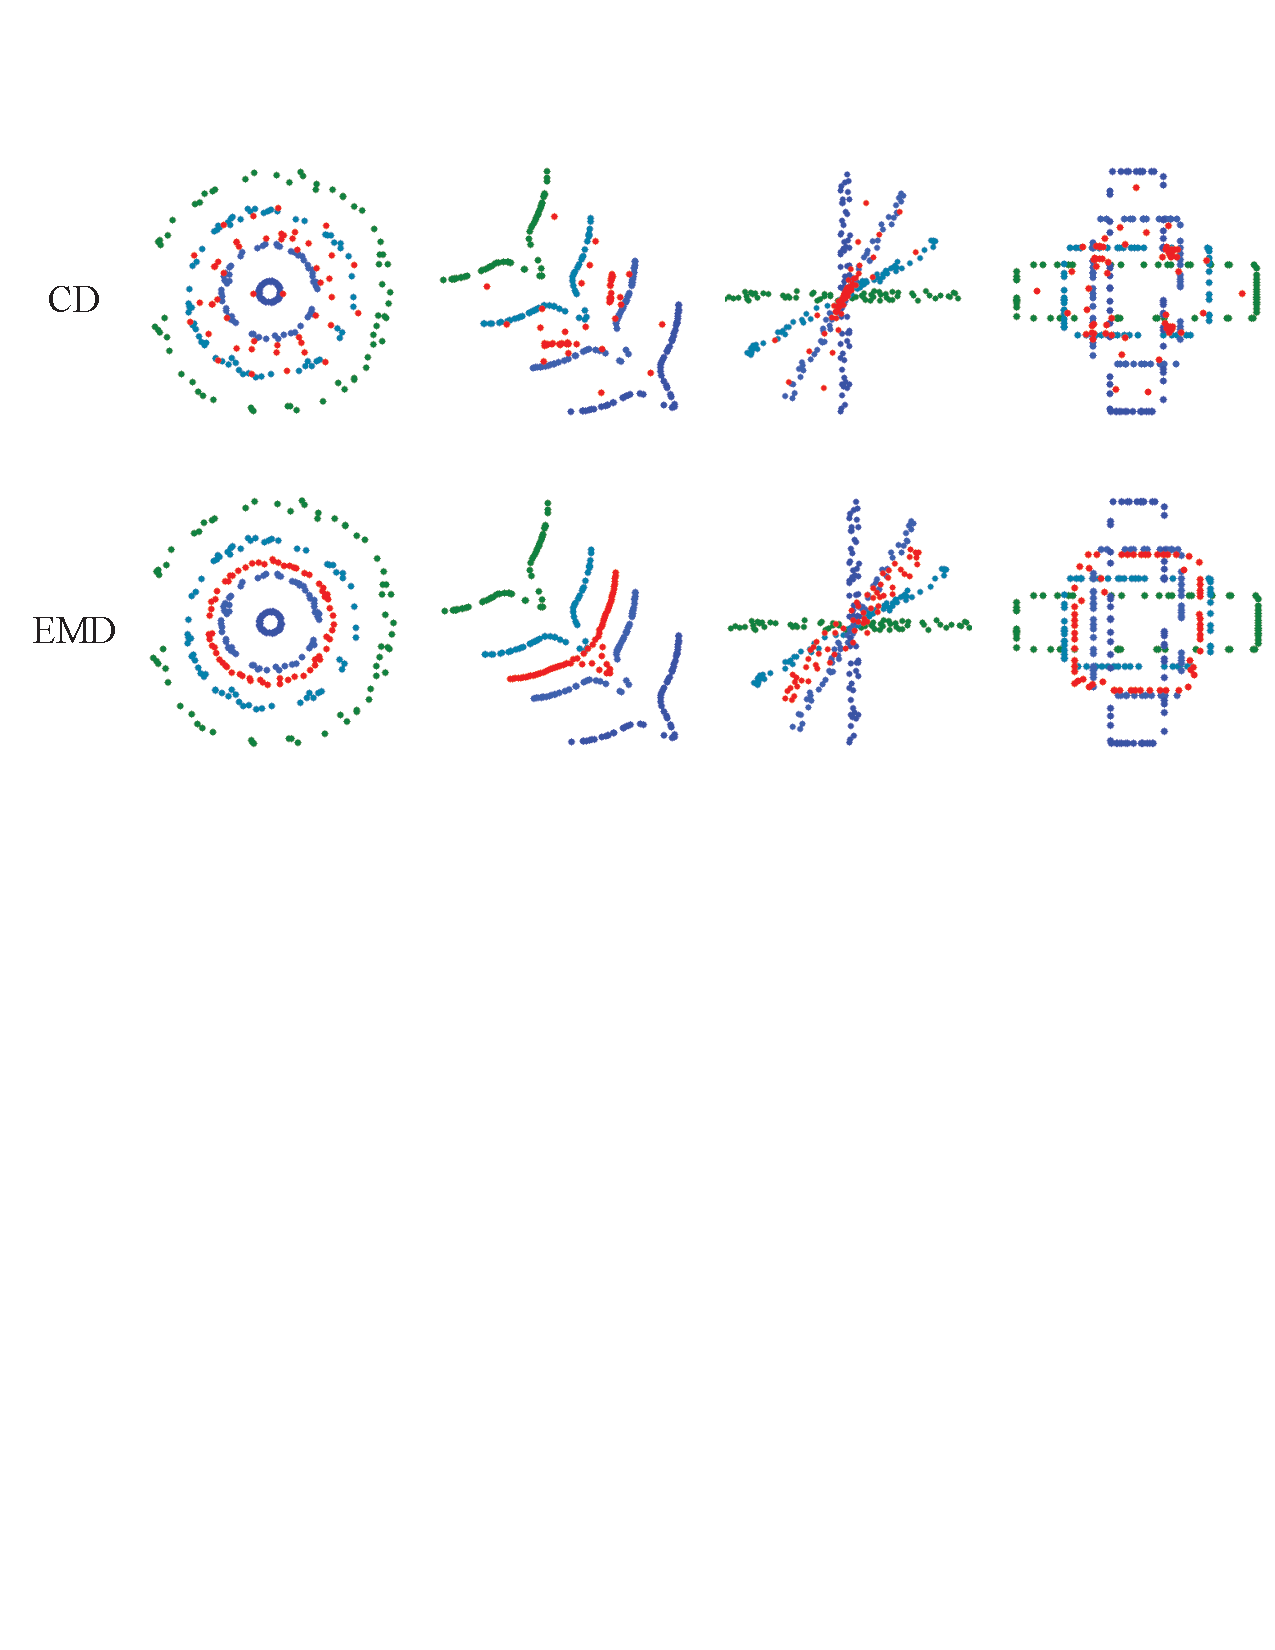
\includegraphics[width=\linewidth]{./fig/interpolation}
  %\caption{The interpolation of point sets by Chamfer distance (CD) versus Earth %Mover's distance (EMD). Each column corresponds to one type of shape. For each %type, we compute the mean shape $E$ (red) from four samples $S_i$ with different %parameters (from green to blue), e.g., radius of a circle. The mean shape is %computed by solving the optimization problem $\min_E \sum_{i=1}^4 d^2(E, S_i)$, %where $d$ can be CD or EMD. We observe that the mean shape from EMD looks more %natural.}
  %\label{fig:interoplation}
%\end{figure}

\paragraph{Shape space}
Despite remarkable expressive power embedded in the deep layers, neural networks inevitably encounter uncertainty in predicting the precise geometry of an object. Such uncertainty could arise from limited network capacity, insufficient use of input resolution, or the ambiguity of groundtruth due to information loss in 3D-2D projection. Facing the inherent inability to resolve the shape precisely, neural networks tend to predict a ``mean'' shape averaging out the space of uncertainty. The mean shape carries the characteristics of the distance itself.

In Figure~\ref{fig:mean}, we illustrate the distinct mean-shape behavior of EMD and CD on synthetic shape distributions, by minimizing
% \begin{equation*}
% \begin{aligned}
% \underset{x}{\mbox{minimize}}&&\mathrm{E}_{s\sim S}[L(x,s)]
% \end{aligned}
% \end{equation*}
$\mathrm{E}_{s\sim \mathbb{S}}[L(x,s)]$
through stochastic gradient descent, where $\mathbb{S}$ is a given shape distribution, $L$ is one of the distance functions. 

In the first and the second case, there is a single continuously changing hidden variable, namely the radius of the circle in (a) and the location of the arc in (b). EMD roughly captures the shape corresponding to the mean value of the hidden variable. In contrast CD induces a splashy shape that blurs the shape's geometric structure. In the latter two cases, there are categorical hidden variables: which corner the square is located at (c) and whether there is a circle besides the bar (d). To address the uncertain presence of the varying part, the minimizer of CD distributes some points outside the main body at the correct locations; while the minimizer of EMD is considerably distorted.

\begin{figure}[t!]
\centering
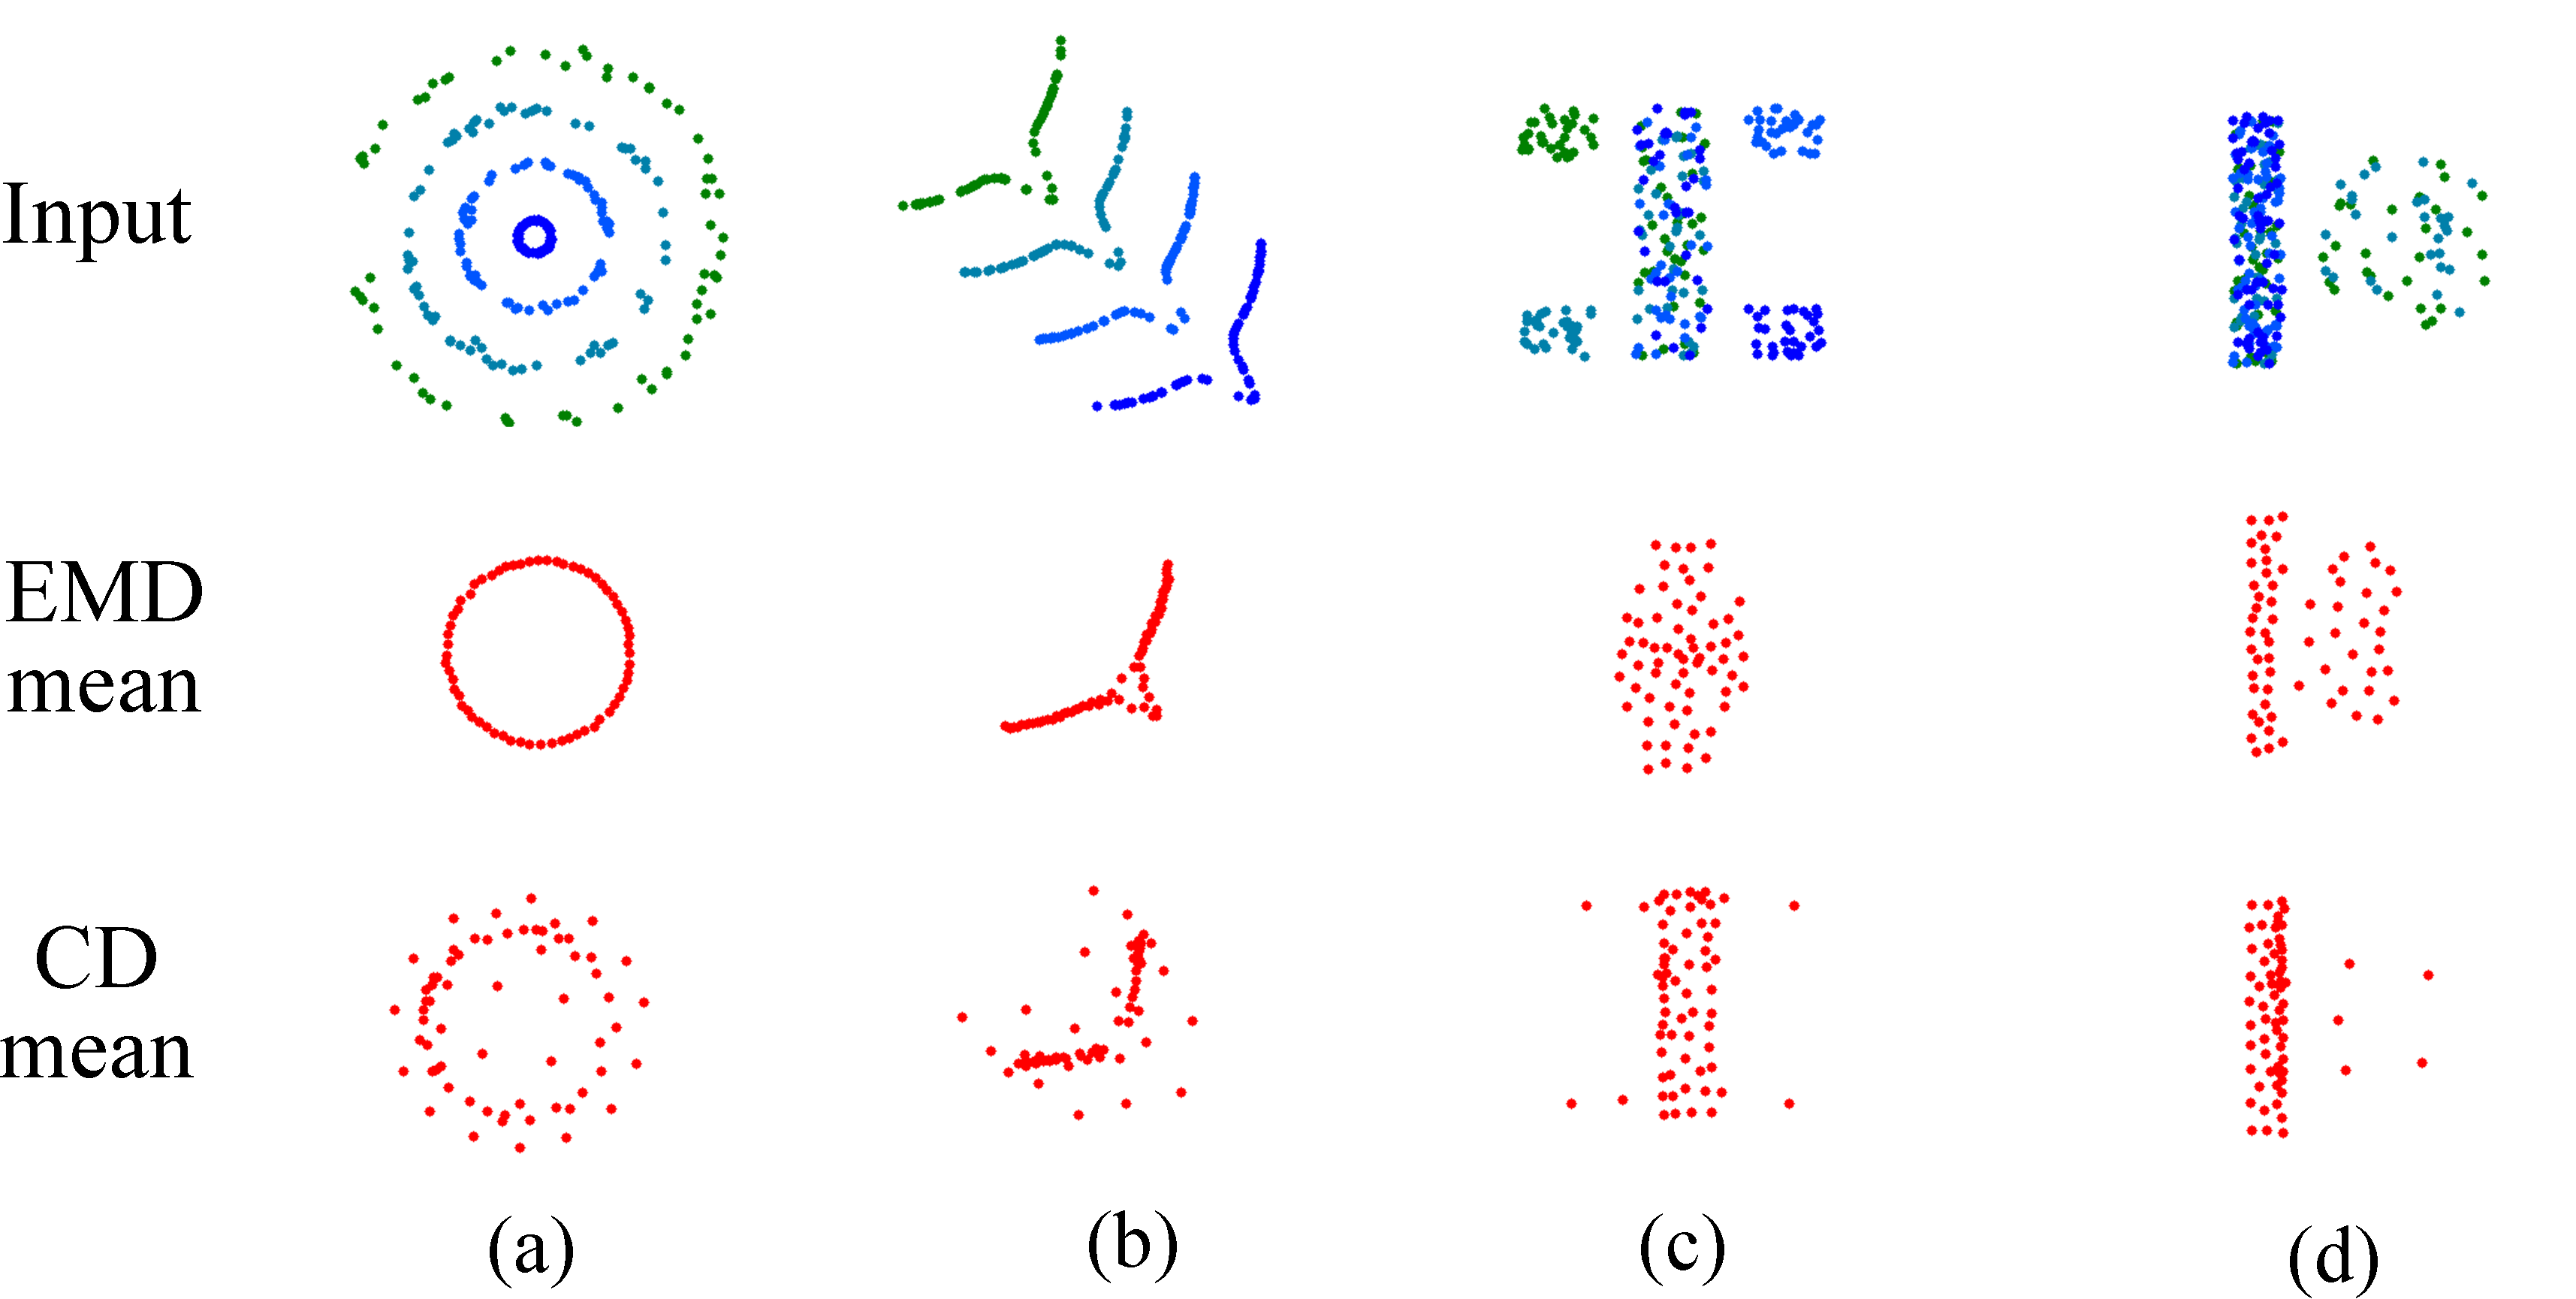
\includegraphics[width=0.9\linewidth]{./fig/show_mean.pdf}
\caption{Mean-shape behavior of EMD and CD. The shape distributions are (a) a circle with varying radius; (b) a spiky arc moving along the diagonal; (c) a rectangle bar, with a square-shaped attachment allocated randomly on one of the four corners; (d) a bar, with a circular disk appearing next to it with probability 0.5. The red dots plot the mean shape calculated according to EMD and CD accordingly.}
\label{fig:mean}
\end{figure}

\subsection{Generation of Multiple Plausible Shapes}
\label{sec:method:gan}
% \todo{
% this is an inherent property of our problem. give an illustrative example to convince the reader.
% 
% therefore, ideally, we should be able to generate the space of plausible shapes. we can think that the gt for each training data is just a sample from the groundtruth space. 
% 
% so we come up with the idea -- make multiple predictions, and at least one of the prediction should match the groundtruth.
% }

Our problem solves an ill-posed problem of 3D structural recovery from a single projection. Posed as a regression problem, ambiguity of the prediction arises at test time -- the depth for visible parts is under-determined, and the geometry for invisible parts has to be hallucinated by guessing. In a statistical view, reasonable predictions from the input image form a distribution.  Reflected in the training set, two images that look alike may have rather different groundtruth shapes. Recall the discussion in the previous section -- the ambiguity of groundtruth shape may significantly affect the trained predictor, as the loss function \eqref{eqn:loss} induces our model to predict the mean of possible shapes.  

\begin{figure}[t!]
  \centering
  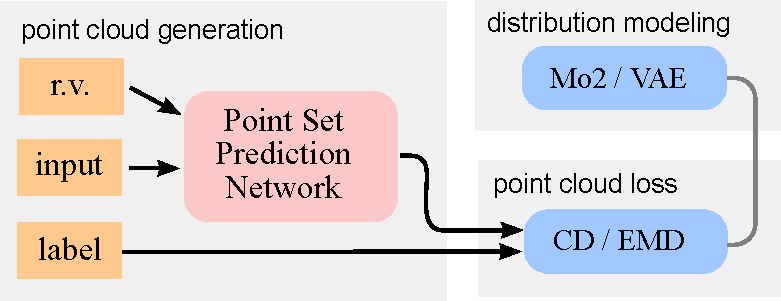
\includegraphics[width=0.8\linewidth]{./fig/system.pdf}
  \caption{System structure. By plugging in distributional modeling module, our system is capable of generating multiple predictions. }
  \label{fig:network}%xiao qiang zhen bang
\end{figure}
%ndeed, the nice interpolation ability of EMD helps us to generate a reasonable mean shape; however, ideally we should fully characterize the landscape of the groundtruth distribution, or be able to sample plausible candidates accordingly. Statistically, we are looking for a conditional sampler dependent on the input image. In this view, the groundtruth shape of each image provided by the training data is in fact a sample from the groundtruth distribution.

To better model the uncertainty or inherent ambiguity (e.g. unseen parts in the single view), we enable the system to generate distributional output. We expect that the random variable $r$ passed to $\mathbb{G}$ (see Eq~\eqref{eqn:main}) would help it explore the groundtruth distribution, in analogy to conditional GAN (CGAN)~\cite{mirza2014conditional}. However, naively plugging $\mathbb{G}$ from Eq~\eqref{eqn:main} into Loss~\eqref{eqn:loss} to predict $S_i^{pred}$ won't work, as the loss minimization will nullify the randomness. It is also unclear how to make CGAN work in our scenario, as building a discriminator that directly consumes a point set is itself an open problem. 

The problem can be solved by more complex frameworks like VAE, where we can incorporate secondary input channels (e.g. another view). However, we find practically a simple and effective method for uncertainty modeling: the MoN loss. We train our network by minimizing a loss function as below:
\begin{equation}
    \begin{aligned}
    \underset{\Theta}{\mbox{minimize}} 
    && 
    \sum_k 
        \min_{
            \substack{r_j\sim \mathbb{N}(\mathbf{0}, \mathbf{I})\\1\le j\le n}
        }
        \{
            d(\mathbb{G}(I_k, r_j;\Theta), S_k^{gt})
        \}
    \end{aligned} 
    \label{eqn:gan}
\end{equation}    

We explain the rationale behind Problem~\eqref{eqn:gan} here. Given an image $I_k$, $\mathbb{G}$ makes $n$ predictions by perturbing the input with $n$ random vectors $r_j$. Intuitively, we expect that one of the predictions will be close to the groundtruth $S_k^{gt}$ given by the training data, meaning that the minimum of the $n$ distances between each prediction and the groundtruth must be small. 

We name this loss as Min-of-N loss (MoN), since it comes from the minimum of $n$ distances. Any of the point set regression networks in Fig~\ref{fig:pointnet} can be plugged into the meta network in Fig~\ref{fig:network} incorporating the MoN loss. In practice, we find that setting $n=2$ already enables our method to well explore the groundtruth space.  Please refer to Sec~\ref{sec:exp:gan} for experiment results.

An alternative way to achieve the conditional shape sampler is by a conditional variational autoencoder. For more details about variational autoencoders, please refer to \cite{doersch2016tutorial}.  Fig~\ref{fig:VAE} shows the system architecture for training and testing a conditional variational autoencoder $P(S|X)$ in our case. Here, $X$ is the input image and $S$ is the \emph{point cloud} representation of the groundtruth 3D shape. At training time, each input image $X$ will be augmented by a random variable that is conditioned on $Y$, which takes the \emph{volumetric} representation of the groundtruth shape $S$. A 3D convolutional network is used as the encoder $Q$ (see \cite{maturana2015voxnet} for a good reference of 3D conv networks). Therefore, a local proximity in the embedding space contains the variations of possible groundtruth 3D shapes.

\begin{figure}
\centering
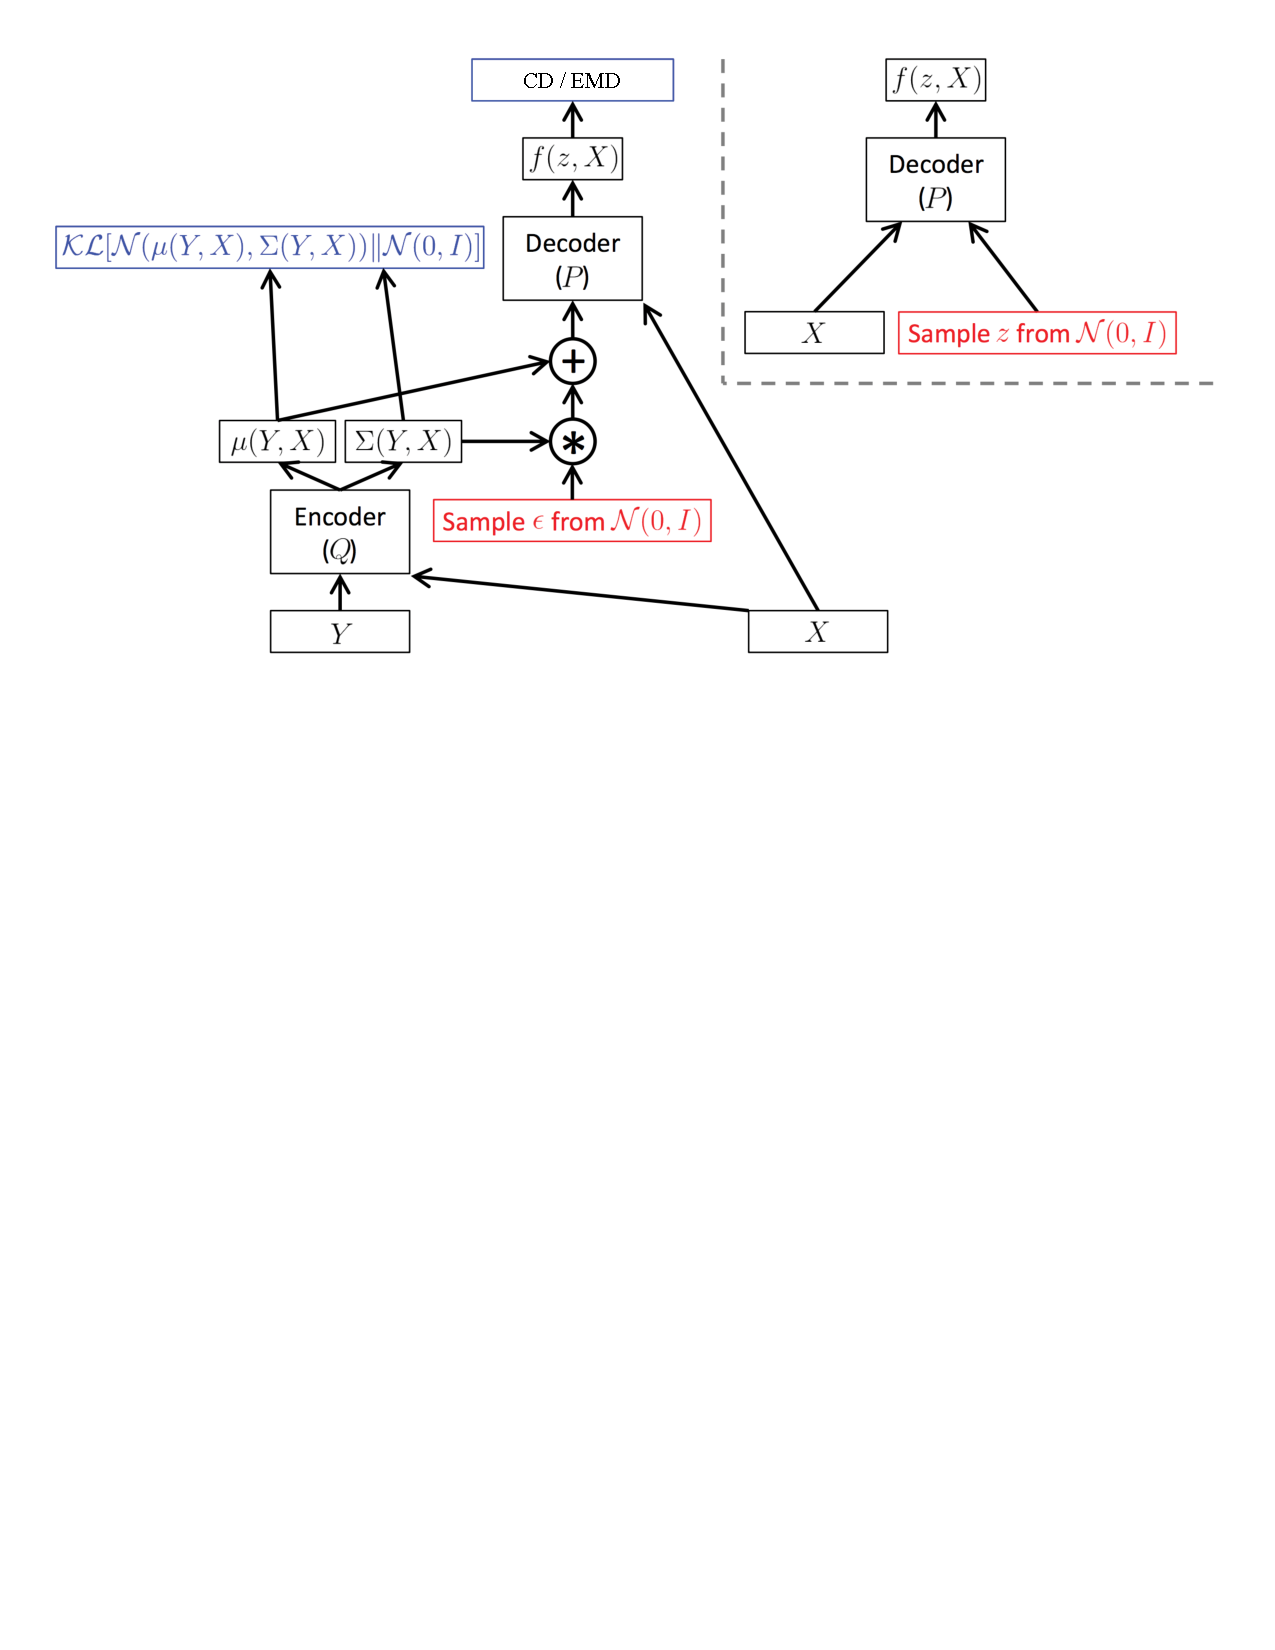
\includegraphics[width=\linewidth]{./fig/vae.pdf}
\caption{Network for conditional variational autoencoder shape sampler $P(S|X)$. Left: a training-time conditional variational autoencoder implemented as a feedforward neural network. Here, $Y$ is the volumetric form of the groundtruth shape $S$, whereas $f(z, X)$ is the point cloud form of the predicted shape for $S$. Right: the same model at test time. (Modified from Doersch et al.~\cite{doersch2016tutorial})}
\label{fig:VAE}
\end{figure}

% An alternative way to build the conditional sampler is through conditional variational autoencoder (VAE) technique, which requires a few additional modules. We explain the VAE version in the supplementary. 



